\chapter{Pogojni stavek}

\section{Zakaj pogojni stavki?}

Vsi programi, ki smo jih do zdaj napisali, so se izvedli po vnaprej določenem zaporedju. Od zgoraj navzdol so se namreč lepo po vrsti izvedli vsi stavki v programu. V določenih primerih pa bi posamezne stavke radi izvedli samo ob izpolnjenosti (ali pa neizpolnjenosti) izbranega pogoja. 

Poglejmo si spodnji primer:
\begin{zgled}
Napiši program, ki od uporabnika prebere telesno težo in višino in izpiše uporabnikov indeks telesne mase.
\end{zgled}
\begin{resitev}
Preko funkcije \texttt{input} bomo torej prebrali težo in višino. Ker funkcija vrača niz, bomo obe vrednosti pretvorili v decimalno število (\texttt{float}). Potem bomo uporabili enačbo za izračun indeksa telesne mase: $itm = \frac{teza}{visina^2}$. Pri tem mora biti teža podana v kilogramih, višina pa v metrih.
\begin{lstlisting}[language=Python,numbers=left]
teza = float(input("Vpisi svojo tezo [kg]: "))
visina = float(input("Vpisi svojo visino [m]: "))
itm = teza/visina**2
print("Tvoj ITM je", itm)
\end{lstlisting}
\end{resitev}

Zgornji program je popolnoma pravilen, bi ga pa radi še malo dopolnili. Veliko uporabnikov verjetno ne ve kaj posamezna vrednost indeksa telesne mase (ITM) pomeni. Ali mora shujšati, je njegova teža ustrezna, ali bi se moral malo zrediti? Če malo poenostavimo, lahko ljudi razdelimo v tri skupine, in sicer tiste s premajhno težo, tiste z ustrezno težo in tiste s preveliko težo:

\begin{tabular}{c|c}
     pogoj & skupina \\
     \hline
     ITM $<$ 18.5 & podhranjenost\\
     18.5 $\leq$ ITM $\leq$ 25 & normalna teža\\
     25 $<$ ITM & debelost
\end{tabular}

Naš program bi torej radi dopolnili tako, da bo uporabniku izpisal tudi informacijo o tem, v katero skupino spada. Z drugimi besedami, če bo izpolnjen prvi pogoj (ITM $<$ 18.5), bi radi izpisali, da je uporabnik podhranjen, če bo izpolnjen drugi pogoj (18.5 $\leq$ ITM $\leq$ 25), da je njegova teža ustrezna in če bo izpolnjen tretji pogoj (25 $<$ ITM), da je pretežak. Radi bi torej, da se določeni deli našega programam (v konkretnem primeru različni izpisi) izvedejo v odvisnosti od vrednosti ITM. 

\section{Osnovna oblika stavka \texttt{if}}

Za pisanje pogojnih stavkov bomo uporabili Pythonov stavek \texttt{if}. Njegova osnovna oblika je sledeča:
\begin{lstlisting}[language=Python]
if pogoj:
    # pogojni_stavki so zamaknjeni
    pogojni_stavek1
    pogojni_stavek2
    ...
# tole se bo izvedlo v vsakem primeru
\end{lstlisting}
Začnemo torej z rezervirano besedico \textbf{\texttt{if}}, ki ji sledi pogoj. Temu sledi dvopičje (\texttt{:}), s katerim povemo, da je konec pogoja. Potem sledi pogojni del, ki se bo izvedel samo v primeru, da je podan pogoj izpolnjen (glej sliko \ref{img:if1}). Pogojnemu delu sledijo stavki, ki se bodo izvedli v vsakem primeru, ne glede na izpolnjenost pogoja. Kako pa Pythonu povemo kje je konec pogojnega dela? Z zamikom \angl{indent}. Zgoraj smo tiste stavke, ki se izvedejo samo v primeru izpolnjenosti pogoja zamaknili, tako da smo pred njih vstavili tabulator (tipka \emph{Tab}) ali par presledkov (če smo pikolovski, se držimo konvencije štirih presledkov). Pogojni del smo zaključili tako, da smo enostano nehali zamikati. Izvedbo zgornje kode prikazuje diagram poteka na sliki \ref{img:if1}.
\begin{figure}
    \centering
    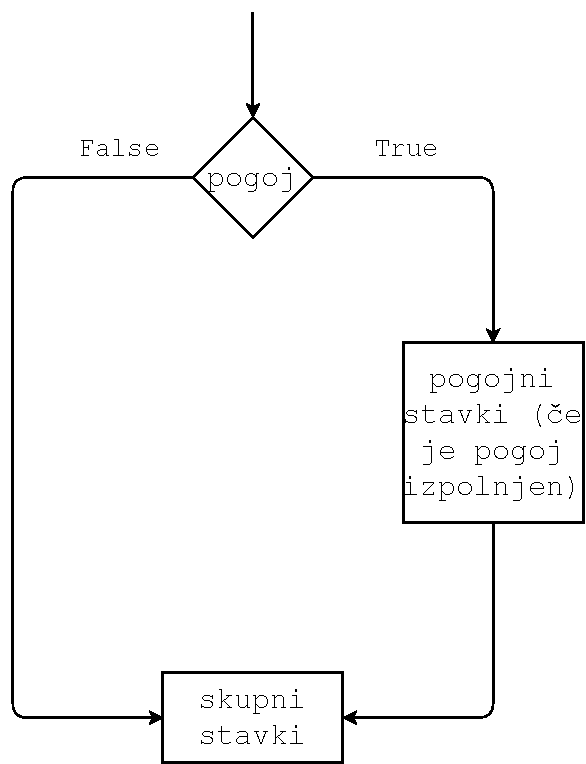
\includegraphics[width=0.5\linewidth]{img/if1.pdf}
    \caption{Diagram poteka osnovne oblike stavka \texttt{if}. V primeru, če je pogoj izpolnjen, se izvede pogojni del.}
    \label{img:if1}
\end{figure}

\section{Kaj lahko nastopa kot pogoj?}

\section{Veja \texttt{else}}


\begin{figure}
    \centering
    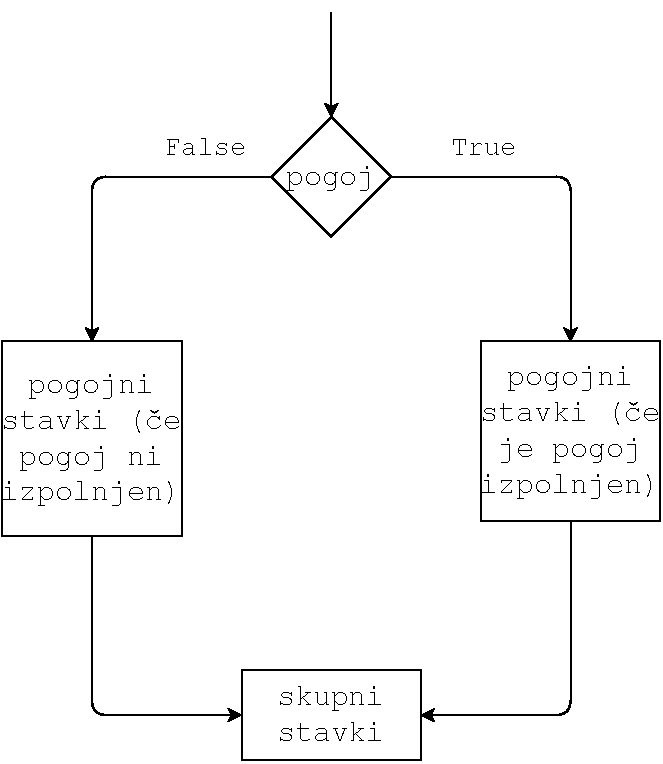
\includegraphics[width=0.5\linewidth]{img/if2.pdf}
    \caption{Caption}
    \label{img:if2}
\end{figure}

\begin{figure}
    \centering
    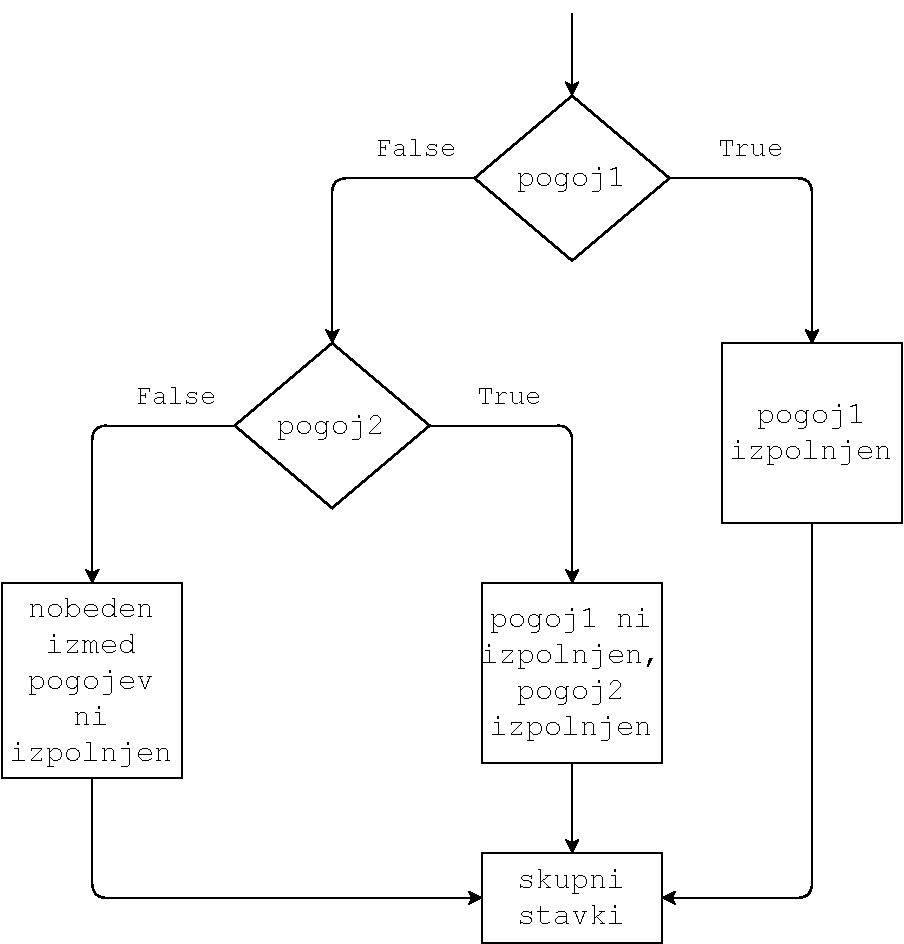
\includegraphics[width=0.65\linewidth]{img/if3.pdf}
    \caption{Caption}
    \label{img:if3}
\end{figure}

\begin{figure}
    \centering
    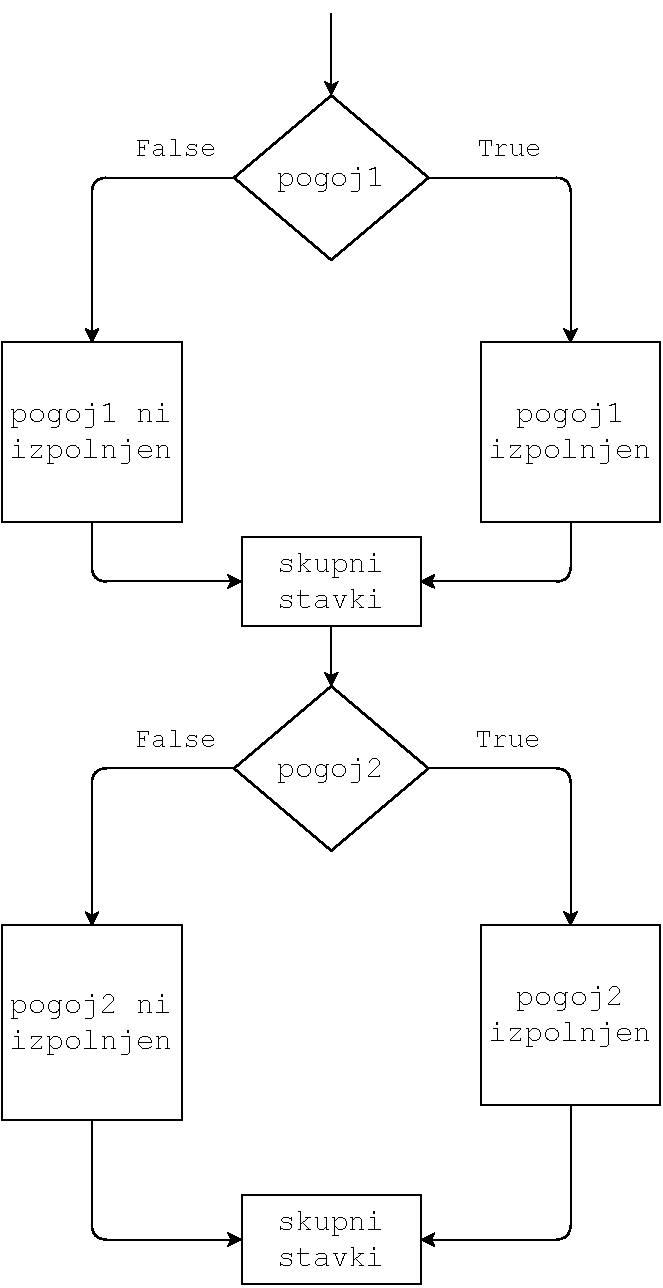
\includegraphics[width=0.5\linewidth]{img/if4.pdf}
    \caption{Caption}
    \label{img:if4}
\end{figure}